\documentclass[]{article}
\usepackage{times}
\usepackage{geometry}
\geometry{margin=1in}
\usepackage{graphicx}
\usepackage{float}
\usepackage{listings}
\usepackage[round]{natbib}
\lstset{
  basicstyle=\fontfamily{lmvtt}\selectfont\small,
  columns=fullflexible,
}

%opening
\title{CS3302 Data Encoding - Adaptive Huffman Coding}
\author{ID: 150013828}

\begin{document}

\maketitle

\section{Overview}
In this practical task we are asked to implement Adaptive Huffman coding, and experiment / evaluate the results. The implementation presented is based heavily on that of \citet{Sayood06}. Presented are also a set of tests on various file / data types as well as a discussion about how well the implementation performs.

\section{Design and Implementation}
I chose to use \emph{C++} to implement the algorithm, and hence I tend to use OOP (loosely) to model the algorithm. Although we see common use of template types in my design, due to complications I have only verified that the classes work (BitReader and BitWriter in particular) for type 'unsigned char' only. My intended use of the template type was to define BitReaders and BitWriters operate on sizes larger than a byte, to see if this affects the compression (I assume it will greatly effect it).
\paragraph{Alphabet} The final implementation supports a single alphabet of size 256 (0-255), as I use bytes to store the symbols.
\paragraph{Node$\langle$T, N$\rangle$} I started by designing a Node class (Node.hpp) as I felt this would be needed in any case. The nodes in question can have any number of children but invariably, due to C++'s template system, a node is only allowed to have children that can have the same number as it can itself. This effectively defines an n-ary tree, but of course, for adaptive Huffman coding we use N as 2 to make a binary tree.
\paragraph{HuffmanTree$\langle$T$\rangle$} The HuffmanTree class contains the root node of the tree, as well as defining other common methods that we need to operate on the tree: \emph{getNTYNode}, \emph{getRoot}, \emph{outputPath}, \emph{findWeightGroup} etc..
\paragraph{NodeData$\langle$T$\rangle$ and Optional$\langle$T$\rangle$} The use of NodeData is mainly just to stop the type signatures of nodes from looking absolutely awful. All nodes in the HuffmanTree class are of type NodeData$\langle$T$\rangle$. NodeData itself is just a struct containing an Optional$\langle$T$\rangle$ as well as a weight value which we need when implementing the algorithm.

Optional is used as a safety guard in this case. In adaptive Huffman coding, only leaf nodes have symbol values associated with them, and hence I use Optional as a non-nullable type in the NodeData struct, we can just check the Optional's \emph{exists} method to check whether or not the value exists, or we should use it. This way, we minimise the amount of dynamic memory allocations in the tree.
\paragraph{HuffmanCoder$\langle$T$\rangle$} Is the base class to HuffmanEncoder and HuffmanDecoder; containing the common structures that both of them need, in particular: a constructor that uses an input stream and and output stream; and the reference to a HuffmanTree.
\paragraph{BitReader$\langle$T$\rangle$ and BitWriter$\langle$T$\rangle$} In order to get a stream of bits, rather than bytes, we abstract over bytes using a bit-buffer. These bit-buffers in particular read in chunks with a size defined by the size of \emph{T}, and feed out/in individual bits. So the use case in the current main file, is as an \emph{unsigned char}, so the buffer size is only a byte in this case.
\paragraph{Particular issues} I had significant issues once I had implemented the algorithm and discovered that the padding around the last byte is a big problem. I.e. when the encoded message does not fit neatly into a multiple of 8 bits, we need to consider: what the encoder should fill those empty places with; and how the decoder should interpret this. Ultimately an issue of making the decoder \emph{stop}!

Initially, to fix the problem, I made it so the encoder would keep a hold of its output stream. Then, in usage, one would call \emph{release} and provide an output stream as the argument. The encoder would then put the length of the stream in bits at the start, and then subsequently pass the rest of its own internal stream to the output stream specified. As great as it might have seemed, this would take away the algorithm's property of \emph{memoryless-ness} - which is one of the key advantages over static Huffman coding algorithms.
\\\\
The solution I found was to just repeatedly output the path to the NYT node as many times as needed to fill any remaining bit places in the output bit-buffer. From the decoder's perspective, it can then read until the input stream reports \emph{EOF}. Then, any remaining bits in the input bit-buffer can either: be decoded as paths to one or more leafs; or if the NYT path happens to be read it can just stop, as there is no possible way of identifying a new symbol after that - it would require at least one buffer's-worth of bits to define.
\\\\
The use of the test scripts was instrumental to finding this EOF error, as it only happened in some files.
\section{Building and Running}
To build the project I use \emph{cmake}. In the project's root directory, run:
\begin{lstlisting}[language=bash]
cmake . && make
\end{lstlisting}
This will generate the executable \emph{huff}. Usage is defined in the file 'README.md', or by running :
\begin{lstlisting}
./huff -h
\end{lstlisting}
The program is always run by specifying an input file, and the desired output name. If the output file already exists it will be \emph{overwritten}.
\paragraph{Tests} To run the tests, simply run:
\begin{lstlisting}
./test.sh <number-of-times-to-repeat>
\end{lstlisting}
Or, to run a specific set of tests, you could run:
\begin{lstlisting}
./testset <location-of-tests> <file-type>
\end{lstlisting}
For example:
\begin{lstlisting}
./testset img bmp
\end{lstlisting}
Runs the canonical test for the compressor over all BMP files in the img directory.
\paragraph{Running compression/decompression}
To compress a file use (with '-r' to generate a report at the end)
\begin{lstlisting}
./huff -r input.txt output.hff
\end{lstlisting}
...and to decompress
\begin{lstlisting}
./huff --puff -r output.hff output.txt
\end{lstlisting}
I should warn though, compression/decompression of larger, more complex images in the 'img' directory can take upwards of two minutes each.
\section{Results and Discussion}
\paragraph{Analysis of the implementation} In order to analyse the compression performance, and to a certain extent the time performance of this Huffman coding algorithm (and to help test correctness in general) I created a series of tests including various file types, sizes, levels of complexity etc..
\subsection{Text files} For text file encoding I included a file containing 50 paragraphs of \emph{lorem ipsum}, and another containing 100; also included is a set of some earlier version of all the source files for this project.

Testing shows that the chosen text files range in compression ratios (compression ratio meaning the percentage of size reduced, rather than the output size as a percentage of the input size) between 23\% and 43\%. The highest compression was gained from the two files containing lorem ipsum, both at 43\%, that is: the compressed output was 57\% of the original size, which is a significant reduction. All of the source code files were consistently less, though varied. I suspect that a reason for this might be that the lorem ipsum files have a limited alphabet than the source code files, hence the tree would be generally smaller, and the codewords.
\subsection{Archive Files} I felt that archive files may have been a good type to investigate as I discovered that they contain a large sequences of very similar data (lots of zeroes, I found). The archive, 'src.tar', which contains all the source files, just as the text example does, achieves a compression of 45\%. Not only is this a sizeable reduction, but it is a higher reduction than we see by combining the reduction percentages by compressing each txt file individually. This is likely because in the compression of each individual file we have to redefine all of the symbols that we see for each file. Whereas, when the directory is in an archive file like this, the symbols only have to be defined once.
\subsection{Image Files} I decided to make some images that contained repeating patterns of various forms, as well as some which do not repeat any discernible pattern (*noise.bmp). The noise images take significantly longer than the other images, despite being the same size. This possibly suggests that creating new nodes in the tree is taking a comparatively longer time, as the noise images will likely have a very wide spread of the available values in the byte alphabet.
\paragraph{Dithering} I took a photo of mine, and created several dithered versions (via a photoshop plugin \footnote[1]{http://www.ximagic.com/cd\_index.html}) of the same image: '*dithered\_N\_boats.bmp'. The higher \emph{N} is, the higher the quality is, a lower value in this case means there are less dithering levels per colour channel - i.e. N is the number of possible values per colour channel.

This is a technique utilized by the GIF image type, used commonly where low bandwidth is a concern. Dithering allows for higher compression by essentially performing some lossy algorithm over the image that means there are less possible values, and this makes the lossless compression better.

\clearpage
\begin{figure}[!htbp]
	\centering
	\begin{minipage}[b]{0.4\textwidth}
		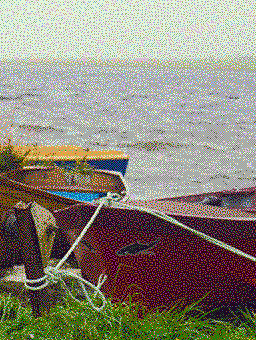
\includegraphics[width=\textwidth]{img/dithering4}
		\caption{4 levels}
	\end{minipage}
	\hfill
	\begin{minipage}[b]{0.4\textwidth}
		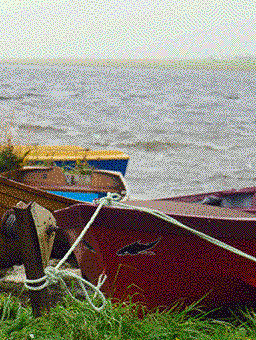
\includegraphics[width=\textwidth]{img/dithering6}
		\caption{6 levels}
	\end{minipage}
\end{figure}
\begin{figure}[!htbp]
	\begin{minipage}[b]{0.4\textwidth}
		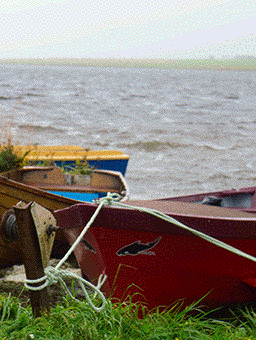
\includegraphics[width=\textwidth]{img/dithering12}
		\caption{12 levels}
	\end{minipage}
	\hfill
	\begin{minipage}[b]{0.4\textwidth}
		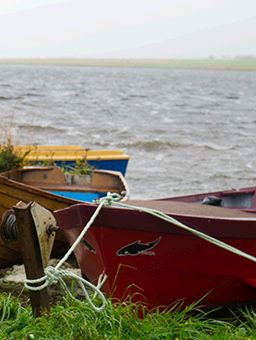
\includegraphics[width=\textwidth]{img/dithering_none}
		\caption{no dithering}
	\end{minipage}
\end{figure}
The compression ratios and compression/decompression times come as no surprise, but I have created some plots based on the output of running the test to try and illustrate some sort of trend (as an average over 5 runs).

\clearpage
\begin{figure}[!htbp]
	\begin{minipage}[b]{\textwidth}
		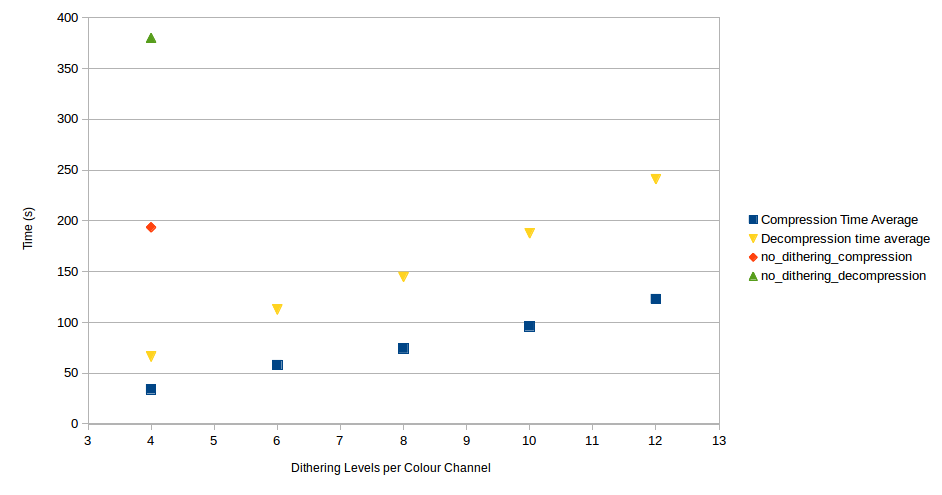
\includegraphics[width=\textwidth]{img/dithering-time}
		\caption{plot of time to compress/decompress against the number of dithering levels. The orange and green points are the values on the y-axis for no dithering.}
	\end{minipage}
	\\\\
	Consider that the orange point ('no\_dithering\_compression') represents the maximum possible time to compress; and the green ('no\_dithering\_decompression') the maximum decompression time - given that we are only varying thee dithering level. It's quite easy to see how successively higher dithering levels would tend towards that value. It looks as though the plot does not show a linear relationship, but we shouldn't be sure until regression analysis is performed.
	
	Notice also how the time to decompress is consistently higher than the time to compress, not only this, but the time of decompression grows faster than to compress. This is useful information; it shows that there is something unique to the decoder in this implementation that has a higher time complexity (or at the very least, a higher coefficient) than the encoding procedure. This could be down to my implementation, or it could be inherent in the algorithm outlined by \citet{Sayood06}.
\end{figure}

\clearpage
\begin{figure}[!htbp]
	\begin{minipage}[b]{\textwidth}
		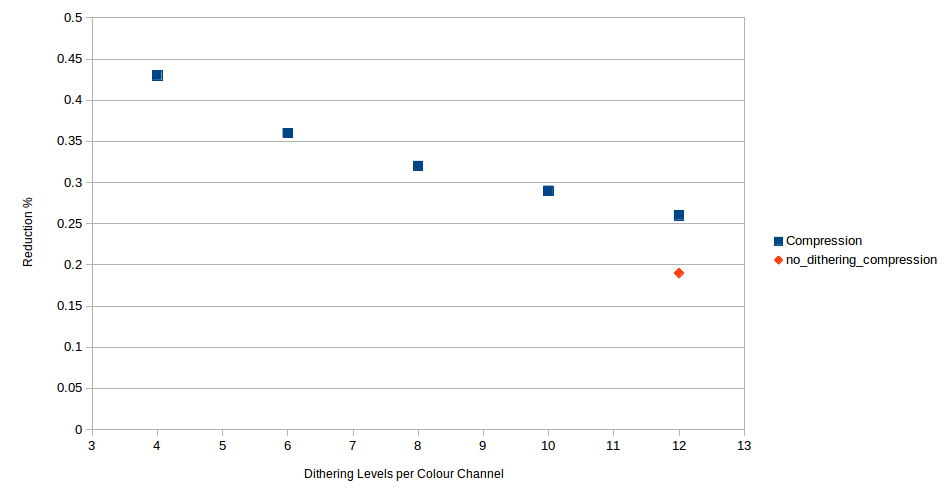
\includegraphics[width=\textwidth]{img/dithering-compression}
		\caption{plot of the level of reduction when compressing against the number of dithering levels. The orange point is the value on the y-axis for no dithering.}
	\end{minipage}
	\\\\
	Likewise, the orange point here ('no\_dithering\_compression') shows the minimum reduction that you can get from the image as the number of dithering levels tends to infinity.
\end{figure}

\clearpage
\section{Evaluation and Conclusion}
\subsection{Evaluation}
\paragraph{Efficiency} Certainly in comparison with most commonly used compression formats, this implementation is very slow. I had attempted to use sound files in my experiments, but even a 4 second wav file was approximately 1.3MB, and took around 20 minutes just to compress.

Areas where the implementation could potentially be faster include:
\begin{itemize}
	\item \emph{reassignIndices} in \emph{HuffmanTree}, for $n$ nodes in the tree, this algorithm is $O(n)$ and is performed after every update to make sure that the indices align with the \emph{sibling property} \citet{Sayood06}. Perhaps there is an invariant that could be exploited after the swapping stage such that we only need to analyse a subsection of nodes.
	\item \emph{findWeightGroup} from \emph{HuffmanTree.hpp} and subsequently \emph{getMaxInWeightGroup} from \emph{FGKTree.hpp}. This is, again, an $O(n)$ operation, and it has to be performed at every update, possibly at each node up the tree.
	It could be that this is too much to ask, but again, perhaps there is an invariant that could be exploited. Perhaps keeping track of nodes with a particular weight?
\end{itemize}
\paragraph{With more time} I would have liked to get the variably typed alphabets working. That way I could experiment with larger sets of symbols, representing larger chunks of data. Which could potentially achieve higher compression.
\subsection{Conclusions}
These experiments show that for this implementation of adaptive Huffman coding:
\begin{itemize}
	\item Adaptive Huffman coding can be made memoryless by repeatedly outputting the NYT path long enough to fill the remaining bits if necessary. The decoder must account for this.
	\item Decoding is consistently slower than encoding.
	\item More varied data also takes consistently longer, this is evident from the time taken to compress/decompress the noise images in comparison to other images of the same size, also with the dithering experiment.
\end{itemize} 
\bibliography{ref}
\bibliographystyle{apalike} 
\end{document}